% !TEX root = task-1-4-3.tex
% Editable task bank. Append new BankTask blocks at the end of the document.
\documentclass[12pt,a4paper]{article}
\usepackage{physics-textbook}
\usepackage{graphicx,needspace}
\usetikzlibrary{decorations.pathmorphing}
\newif\ifShowSolutions
\ifdefined\TutorEdition
  \ShowSolutionstrue
\else
  \ShowSolutionsfalse % Change to \ShowSolutionstrue to display solutions.
\fi
\newcounter{banktask}
\newsavebox{\BankTaskBox}
\newcommand{\BankTaskContent}[3]{%
  \noindent\textbf{\thebanktask.}\quad #2\par
  \ifShowSolutions
    \Needspace{50mm}% Keep the solution heading with its opening text or diagram.
    #3\par
    \ifdefined\TutorEdition
      \ifcsname TutorSource#1\endcsname
        \nopagebreak\smallskip{\small\csname TutorSource#1\endcsname\par}%
      \fi
    \fi
  \fi
}
\newcommand{\BankTask}[3]{%
  \refstepcounter{banktask}\par\medskip
  \sbox{\BankTaskBox}{\begin{minipage}{\linewidth}%
    \BankTaskContent{#1}{#2}{#3}\end{minipage}}%
  \ifdim\dimexpr\ht\BankTaskBox+\dp\BankTaskBox\relax>\dimexpr\textheight-20mm\relax
    \Needspace{35mm}\BankTaskContent{#1}{#2}{#3}%
  \else
    \Needspace{\dimexpr\ht\BankTaskBox+\dp\BankTaskBox\relax}%
    \noindent\usebox{\BankTaskBox}\par
  \fi
  \medskip
}
\begin{document}
\BookSubsection{1.4.3}{Центростремительное ускорение}


% Source sdamgia-129: https://phys-ege.sdamgia.ru/problem?id=129
\BankTask{sdamgia-129}{
Материальная точка равномерно движется со скоростью $u$ по окружности радиусом r. Как изменится модуль ее центростремительного ускорения, если скорость точки будет вдвое больше?

$1$) не изменится

$2$) уменьшится в $2$ раза

$3$) увеличится в $2$ раза

$4$) увеличится в $4$ раза
}{
\smallskip\noindent\textbf{Решение}\par
Центростремительное ускорение дается следующим выражением: $a= \frac{u ^2}{r} ,$ оно пропорционально квадрату скорости движения материальной точки по окружности. Если скорость материальной точки будет вдвое больше, то модуль ее центростремительного ускорение увеличится в $4$ раза.

Ответ: $4$.
}

% Source sdamgia-3097: https://phys-ege.sdamgia.ru/problem?id=3097
\BankTask{sdamgia-3097}{
Материальная точка движется по окружности радиуса $R$. Что произойдет с периодом, частотой обращения и центростремительным (нормальным) ускорением точки при увеличении линейной скорости движения в $2$ раза?

К каждому элементу первого столбца подберите соответствующий элемент из второго и внесите в строку ответов выбранные цифры под соответствующими буквами.

\TaskMatchingColumns{Физические величины}{А) Период обращения материальной точки\par 
Б) Частота обращения материальной точки\par 
В) Центростремительное (нормальное) ускорение материальной точки}{Изменение величины}{$1$. Увеличится\par 
$2$. Уменьшится\par 
$3$. Не изменится}

\begin{center}\small\renewcommand{\arraystretch}{1.25}\begin{tabular}{|p{0.300\linewidth}|p{0.300\linewidth}|p{0.300\linewidth}|}\hline
$A$ & Б & В\\\hline
 &  & \\\hline
\end{tabular}\end{center}
}{
\smallskip\noindent\textbf{Решение}\par
Период обращения материальной точки по окружности связан с радиусом окружности и скоростью движения соотношением $T= \frac{2 \pi  R}{v} .$ Следовательно, при увеличении скорости движения период обращения уменьшится (А — $2$). Частота обратно пропорциональна периоду, значит, частота увеличится (Б — $1$). Центростремительное (нормальное) ускорение прямо пропорционально квадрату скорости: $a_{\text{ц}}= \frac{v ^2}{R} .$ Таким образом, увеличение скорости приведет к увеличению центростремительного ускорения (В — $1$).

Ответ: $211$.
}

% Source sdamgia-5145: https://phys-ege.sdamgia.ru/problem?id=5145
\BankTask{sdamgia-5145}{
Материальная точка движется по окружности радиусом $R$ со скоростью $v .$ Как нужно изменить скорость ее движения, чтобы при увеличении радиуса окружности в $2$ раза центростремительное ускорение точки осталось прежним?

$1$) увеличить в $2$ раза

$2$) уменьшить в $2$ раза

$3$) увеличить в $\sqrt{2}$ раза

$4$) уменьшить в $\sqrt{2}$ раза
}{
\smallskip\noindent\textbf{Решение}\par
Центростремительное ускорение связано со скоростью движения и радиусом окружности соотношением

\[a= \frac{v ^2}{R}\]

Таким образом, для того, чтобы при увеличении радиуса окружности в $2$ раза, центростремительное ускорение точки осталось неизменным, скорость необходимо увеличить в $\sqrt{2}$ раза.

Ответ: $3$
}

% Source sdamgia-6188: https://phys-ege.sdamgia.ru/problem?id=6188
\BankTask{sdamgia-6188}{
Верхнюю точку моста радиусом $100\,\text{м}$ автомобиль проходит со скоростью $20\,\text{м/с}$. Чему равно центростремительное ускорение автомобиля? (Ответ дайте в метрах в секунду в квадрате.)
}{
\smallskip\noindent\textbf{Решение}\par
Центростремительное ускорение равно

\[a_{\text{ц}}= \frac{v ^2}{R} = \frac{400}{100} =4\,\text{м/с} ^2 .\]

Ответ: $4$.
}

% Source sdamgia-6260: https://phys-ege.sdamgia.ru/problem?id=6260
\BankTask{sdamgia-6260}{
Груз, подвешенный на нити длиной $2\,\text{м}$, отведен в сторону и отпущен. Нижнюю точку траектории он проходит со скоростью $1{,}4\,\text{м/с}$. Найдите центростремительное ускорение груза в нижней точке траектории. (Ответ дайте в метрах в секунду в квадрате и округлите до целых.)
}{
\smallskip\noindent\textbf{Решение}\par
Центростремительное ускорение равно

\[a_{\text{ц}}= \frac{v ^2}{R} = \frac{1{,}4 ^2}{2} \approx1\,\text{м/с} ^2 .\]

Ответ: $1$.
}

% Source sdamgia-23230: https://phys-ege.sdamgia.ru/problem?id=23230
\BankTask{sdamgia-23230}{
Ускорение свободного падения на поверхности некоторой сферической однородной планеты равно $g$, а первая космическая скорость для этой планеты равна $v _1.$ Установите соответствие между физическими величинами и формулами, при помощи которых их можно вычислить. 

\TaskMatchingColumns{Физическая величина}{А) радиус планеты\par 
Б) модуль центростремительного ускорения \par 
спутника, летающего вокруг планеты на высоте h \par 
над ее поверхностью по круговой орбите}{Формула}{$1$) $\frac{gv_1^4}{(v_1^2+gh)^2}$\par 
$2$) $\frac{v _1 ^2}{2g}$\par 
$3$) $\frac{v _1 ^2}{g}$\par 
$4$) $\frac{g v _1 ^2}{v _1 ^2 + gh}$}

\begin{center}\small\renewcommand{\arraystretch}{1.25}\begin{tabular}{|p{0.450\linewidth}|p{0.450\linewidth}|}\hline
А & Б\\\hline
 & \\\hline
\end{tabular}\end{center}
}{
\smallskip\noindent\textbf{Решение}\par
А) Из формулы первой космической скорости $v _1= \sqrt{gR}$ найдем радиус планеты: $R= \frac{v _1 ^2}{g} .$

Б) Из равенства сил $F = ma_{\text{ц}}c = \frac{m v ^2}{R + h}$ и $F_{\text{т}}=G \frac{Mm}{( R + h ) ^2} ,$ находим, что: 

\[v ^2 = \frac{GM}{R + h} ,\]

откуда:

\[a_{\text{цс}}=\frac{F_{\text{т}}}{m}=\frac{GM}{(R+h)^2}=\frac{v_1^4}{g(R+h)^2}=\frac{v_1^4g}{(v_1^2+gh)^2}.\]

Ответ: $31$.
}

% Source sdamgia-28081: https://phys-ege.sdamgia.ru/problem?id=28081
\BankTask{sdamgia-28081}{
В школьном опыте брусок, помещенный на горизонтальный диск, вращается вместе с ним с некоторой угловой скоростью. В ходе опыта угловую скорость диска увеличили. При этом положение бруска на диске осталось прежним. Как изменились при этом центростремительное ускорение бруска и сила трения между бруском и опорой? 

Для каждой величины определите соответствующий характер изменения.

$1$. Увеличилась.

$2$. Уменьшилась.

$3$. Не изменилась.

 

\begin{center}\small\renewcommand{\arraystretch}{1.25}\begin{tabular}{|p{0.450\linewidth}|p{0.450\linewidth}|}\hline
Центростремительное

ускорение бруска & Сила трения между бруском

и опорой\\\hline
 & \\\hline
\end{tabular}\end{center}
}{
\smallskip\noindent\textbf{Решение}\par
Центростремительное ускорение бруска $a=\omega ^2 R.$ При увеличении угловой скорости центростремительное ускорение увеличивается ($1$). Так как брусок остается на месте, то сила трения $F_{mp}=ma,$ значит, сила трения также увеличилась ($1$).

Ответ: $11$.
}

% Source sdamgia-32242: https://phys-ege.sdamgia.ru/problem?id=32242
\BankTask{sdamgia-32242}{
Небольшое тело движется по окружности радиусом $R$ с линейной скоростью $\upsilon $. Во сколько раз увеличится центростремительное ускорение тела, если его скорость увеличилась в $3$ раза?
}{
\smallskip\noindent\textbf{Решение}\par
Зависимость центростремительного ускорения от скорости имеет вид $a= \frac{v ^2}{R} .$ Из формулы следует, что при увеличении скорости в $3$ раза центростремительное ускорение увеличится в $9$ раз.

Ответ: $9$.
}

% Source sdamgia-35161: https://phys-ege.sdamgia.ru/problem?id=35161
\BankTask{sdamgia-35161}{
Шарик движется по окружности радиусом $R$ с угловой скоростью \ensuremath{\omega}. Во сколько раз уменьшится центростремительное ускорение шарика, если радиус окружности увеличить вдвое, а угловую скорость уменьшить в $2$ раза?
}{
\smallskip\noindent\textbf{Решение}\par
Центростремительное ускорение определяется по формуле $a=\omega ^2 R.$ При увеличении радиуса в $2$ раза центростремительное ускорение увеличится в $2$ раза; при уменьшении угловой скорости в $2$ раза центростремительное ускорение уменьшится в $4$ раза. В результате ускорение уменьшится в $2$ раза.

Ответ: $2$.
}

% Source sdamgia-51358: https://phys-ege.sdamgia.ru/problem?id=51358
\BankTask{sdamgia-51358}{
Вокруг Земли по круговой орбите вращается искусственный спутник. В результате перехода на другую круговую орбиту центростремительное ускорение спутника уменьшилось. Как изменились в результате этого перехода частота обращения спутника вокруг Земли и скорость его движения по орбите?

Для каждой величины определите соответствующий характер ее изменения.

$1$. Увеличится.

$2$. Уменьшится.

$3$. Не изменится.

 

\begin{center}\small\renewcommand{\arraystretch}{1.25}\begin{tabular}{|p{0.450\linewidth}|p{0.450\linewidth}|}\hline
Частота обращения спутника 

вокруг Земли & Скорость движения 

спутника по орбите\\\hline
 & \\\hline
\end{tabular}\end{center}
}{
\smallskip\noindent\textbf{Решение}\par
На спутник действует сила тяжести, равная $F=G \frac{mM}{R ^2} ,$ под действием которой он движется с ускорением свободного падения 

\[a = g = \frac{F}{m} = G \frac{M}{R ^2} .\]

 При уменьшении ускорения спутника радиус орбиты увеличивается. 

Спутник движется со скоростью 

\[v = \sqrt{aR} = \sqrt{G \frac{M}{R}} .\]

 При увеличении радиуса орбиты скорость спутника уменьшается ($2$).

Период обращения спутника равен: 

\[T = \frac{2 \pi  R}{v} = 2 \pi  R \sqrt{\frac{R}{GM}} .\]

 При увеличении радиуса орбиты период обращения спутника увеличивается, а частота обращения $\nu = \frac{1}{T}$ уменьшается ($2$).

Ответ: $22$.
}


% Source 3A9974: https://ege.fipi.ru/bank/questions.php?search=1&proj=BA1F39653304A5B041B656915DC36B38&qid=3A9974
\BankTask{3A9974}{
Грузовик массой $10\,\text{т}$ проезжает верхнюю точку выпуклого моста, радиус кривизны которого равен $80\,\text{м}$, двигаясь равномерно со скоростью $72\,\text{км}/\text{ч}$.
\begin{enumerate}
\item Сила тяжести, действующая на грузовик, равна $10\,\text{кН}$.
\item Сумма сил, действующих на грузовик, направлена вертикально вверх и перпендикулярна его скорости.
\item Центростремительное ускорение грузовика равно $5\,\text{м}/\text{с}^{2}$.
\item Сила, с которой мост действует на грузовик, меньше $40\,\text{кН}$ и направлена вертикально вверх.
\item Сила, с которой грузовик действует на мост, направлена вертикально вниз и равна $50\,\text{кН}$.
\end{enumerate}
}{
\smallskip\noindent\textbf{Решение от GPT}\par
$m=10^4\,\text{кг}$, $v=20\,\text{м}/\text{с}$. Ускорение $a=v^2/R=5\,\text{м}/\text{с}^2$ направлено вниз. $mg=100\,\text{кН}$, $N=m(g-a)=50\,\text{кН}$ направлена вверх; на мост грузовик действует вниз с той же силой. Ответ: $35$.
}

% Source F4D3FF: https://ege.fipi.ru/bank/questions.php?search=1&proj=BA1F39653304A5B041B656915DC36B38&qid=F4D3FF
\BankTask{F4D3FF}{
Космический аппарат, обращающийся вокруг Луны по круговой орбите, перешёл на другую круговую орбиту бóльшего радиуса. Как изменились в результате этого перехода центростремительное ускорение, с которым аппарат движется по орбите, и его период обращения вокруг Луны?
\begin{enumerate}
\item увеличилась
\item уменьшилась
\item не изменилась
\end{enumerate}
\TaskChangeTable{Центростремительное ускорение}{Период обращения аппарата вокруг Луны}
}{
\smallskip\noindent\textbf{Решение от GPT}\par
$a=GM/r^2$ уменьшается с ростом радиуса; $T=2\pi\sqrt{r^3/(GM)}$ увеличивается. Ответ: $21$.
}

% Source FcA2F2: https://ege.fipi.ru/bank/questions.php?search=1&proj=BA1F39653304A5B041B656915DC36B38&qid=FcA2F2
\BankTask{FcA2F2}{
В школьном опыте брусок, помещённый на горизонтальный диск, вращался вместе с ним с некоторой угловой скоростью. В ходе опыта угловую скорость диска увеличили. При этом положение бруска на диске осталось прежним. Как изменились при этом центростремительное ускорение бруска и сила нормального давления бруска на опору?
\begin{enumerate}
\item увеличилась
\item уменьшилась
\item не изменилась
\end{enumerate}
\TaskChangeTable{Центростремительное ускорение бруска}{Сила нормального давления бруска на опору}
}{
\smallskip\noindent\textbf{Решение от GPT}\par
$a=\omega^2r$ увеличивается. По вертикали ускорения нет, поэтому сила нормального давления $N=mg$ не меняется. Ответ: $13$.
}

% Source 29806: https://phys-ege.sdamgia.ru/problem?id=29806
\BankTask{29806}{
\begin{center}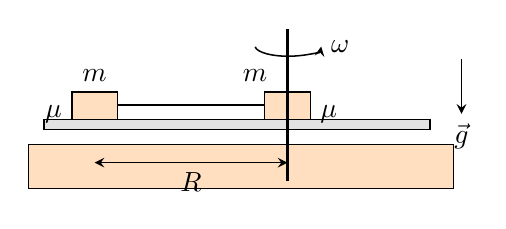
\begin{tikzpicture}[>=stealth,line width=.55pt]\draw[fill=orange!25](-.2,-.75)rectangle(5.2,-.19);\draw[fill=gray!22](0,0)rectangle(4.9,.13);\draw[fill=orange!25](.35,.13)rectangle(.93,.48) (2.8,.13)rectangle(3.38,.48);\draw[thick](3.09,-.65)--(3.09,1.28);\draw(.93,.31)--(2.8,.31);\draw[->](2.68,1.05)arc(185:357:.42 and .13)node[right]{$\omega$};\node[above]at(.64,.48){$m$};\node[above left]at(2.96,.48){$m$};\node[left]at(.35,.19){$\mu$};\node[right]at(3.38,.2){$\mu$};\draw[<->](.64,-.42)--(3.09,-.42)node[midway,below]{$R$};\draw[->](5.3,.9)--(5.3,.2)node[below]{$\vec g$};\end{tikzpicture}\end{center} На горизонтальный диск проигрывателя пластинок положили два одинаковых маленьких грузика массой m каждый, соединенных между собой горизонтальной нитью, один  — в центре, другой  — на расстоянии R  =  $12\,\text{см}$ от оси вращения (см. рисунок). Коэффициенты трения грузиков о диск одинаковы и равны $\mu=0{,}4.$ Диск начали вращать, медленно увеличивая его угловую скорость. При каком значении частоты $v$ вращения грузики свалятся с диска? Считайте, что нить невесома, нерастяжима и вначале не была натянута.
}{
\smallskip\noindent\textbf{Решение}\par
\begin{center}\begin{tikzpicture}[>=stealth,line width=.55pt]\draw[fill=orange!25](-.2,-.75)rectangle(5.2,-.19);\draw[fill=gray!22](0,0)rectangle(4.9,.13);\draw[fill=orange!25](.35,.13)rectangle(.93,.48) (2.8,.13)rectangle(3.38,.48);\draw[thick](3.09,-.65)--(3.09,1.28);\draw(.93,.31)--(2.8,.31);\draw[->](2.68,1.05)arc(185:357:.42 and .13)node[right]{$\omega$};\draw[->](.64,.31)--(.64,1.16)node[above]{$\vec N$};\draw[->](3.09,.31)--(3.09,1.16)node[above]{$\vec N$};\draw[->](.64,.31)--(.64,-.63)node[below]{$m\vec g$};\draw[->](3.09,.31)--(3.09,-.63)node[below]{$m\vec g$};\draw[->](.64,.31)--(1.61,.31)node[above]{$\vec T$};\draw[->](3.09,.31)--(2.12,.31)node[above]{$\vec T$};\draw[->](.64,.13)--(1.57,.13)node[below]{$\vec F_{\text{тр}1}$};\draw[->](3.09,.13)--(4,.13)node[above]{$\vec F_{\text{тр}2}$};\end{tikzpicture}\end{center}$1$.  Проанализируем процессы, происходящие в системе при раскручивании диска проигрывателя, изобразив силы, действующие при этом на грузики (см. рисунок). Силы натяжения, действующие на каждый груз, равны по модулю в силу невесомости нити.
$2$.  До начала раскручивания все тела находятся в покое, и сумма сил, действующих на грузики по вертикали и по горизонтали, равна нулю. Силы нормального давления N грузиков на диск и диска на грузики, одинаковые по третьему закону Ньютона, равны весам грузиков: N  =  mg. Это же соотношение выполняется и после начала раскручивания диска. 
$3$.  После начала медленного раскручивания первый грузик приобретает центростремительное ускорение $a=4 \pi ^2 \nu ^2 R,$ которое возникает по второму закону Ньютона за счет действия силы трения покоя $F_{\,\text{тр}}1 < \,\text{или} \,\text{равно} \mu N=\mu mg,$ откуда $m\omega ^2 R < \,\text{или} \,\text{равно} \mu mg.$
$4$.  В момент достижения предельного значения силы трения покоя первый грузик сдвигается и натягивает нить, то есть появляется сила натяжения нити T, действующая также и на второй грузик и возрастающая по мере ускорения вращения диска. При этом центральный грузик будет оставаться на месте, и $T=F_{\,\text{тр}}2 < \,\text{или} \,\text{равно} \mu N=\mu mg.$
$5$.  Это происходит с ростом $\omega$ до тех пор, пока сила трения $F_{\,\text{тр}}2$ не достигнет своего предельного значения $\mu mg=T_{\,\text{м}},$ после чего второй грузик начнет скользить от оси вращения, и оба грузика свалятся с диска.
$6$.  В момент начала скольжения центрального грузика по диску уравнение движения первого грузика имеет вид: $4 \pi ^2 \nu ^2 Rm=T_{\,\text{м}} + \mu mg=2\mu mg,$ откуда частота вращения диска:

\[\nu = \frac{1}{2 \pi} \sqrt{\frac{2\mu g}{R}} = \frac{1}{2 \cdot 3{,}14} \cdot \sqrt{\frac{2 \cdot 0{,}4 \cdot 10}{0{,}12}} \approx 1{,}3\,\text{Гц}.\]

Ответ: $\approx 1{,}3\,\text{Гц}.$
}

% Source 38971: https://phys-ege.sdamgia.ru/problem?id=38971
\BankTask{38971}{
\begin{center}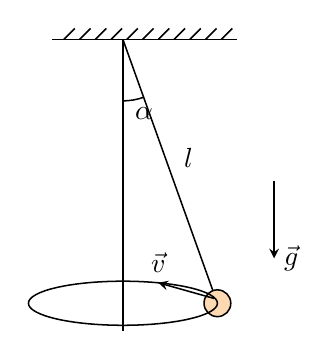
\begin{tikzpicture}[>=stealth,line width=.55pt]\draw(-.9,3.35)--(1.45,3.35);\foreach \x in {-.75,-.55,...,1.25}{\draw(\x,3.35)--++(.14,.14);}\draw(0,3.35)--(0,-.35);\draw(0,3.35)--(1.2,0);\draw(0,2.57)arc(-90:-70:.78)node[below]{$\alpha$};\draw[fill=orange!30](1.2,0)circle(.17);\draw(0,0)ellipse(1.2 and .28);\node[right]at(.65,1.85){$l$};\draw[->](1.16,.06)--(.45,.26)node[above]{$\vec v$};\draw[->](1.92,1.55)--(1.92,.57)node[right]{$\vec g$};\end{tikzpicture}\end{center}Небольшой груз, прикреплённый к нити длиной l  =  $15\,\text{см}$, вращается вокруг вертикальной оси так, что нить отклоняется от вертикали на угол $\alpha$  =  $60$°. С какой скоростью движется груз?
}{
\smallskip\noindent\textbf{Решение}\par
\begin{center}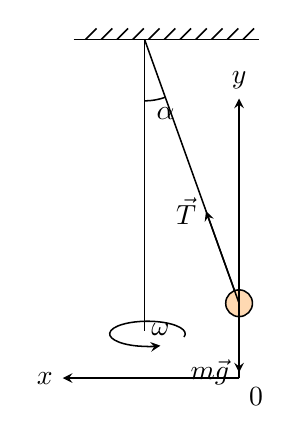
\begin{tikzpicture}[>=stealth,line width=.55pt]\draw(-.9,3.35)--(1.45,3.35);\foreach \x in {-.75,-.55,...,1.25}{\draw(\x,3.35)--++(.14,.14);}\draw(0,3.35)--(0,-.35);\draw(0,3.35)--(1.2,0);\draw(0,2.57)arc(-90:-70:.78)node[below]{$\alpha$};\draw[fill=orange!30](1.2,0)circle(.17);\draw[->](1.2,-.95)--(-1.04,-.95)node[left]{$x$};\draw[->](1.2,-.95)--(1.2,2.6)node[above]{$y$};\node[below right]at(1.2,-.95){$0$};\draw[->](1.2,0)--(.78,1.17)node[left]{$\vec T$};\draw[->](1.2,0)--(1.2,-.88)node[left]{$m\vec g$};\draw[->](.5,-.43)arc(-15:290:.48 and .16)node[above]{$\omega$};\end{tikzpicture}\end{center}Изобразим силы, действующие на грузик. По второму закону Ньютона в ИСО $\overrightarrow{T} + m \vec{g} = m \vec{a},$ где m  — масса грузика, T  — сила натяжения нити. В проекциях на координатные оси получаем:

$Ox: T \sin \alpha = ma,$
$Oy: T \cos \alpha = mg.$

 Следовательно, центростремительное ускорение грузика $a = g \tan \alpha .$ При равномерном движении по окружности со скоростью \ensuremath{\upsilon} по окружности радиусом $R = l \sin \alpha$ грузик имеет центростремительное ускорение $a = \frac{v ^2}{R} .$ Таким образом, скорость, с которой движется грузик, равна

\[v = \sqrt{\frac{gl \sin ^2 \alpha}{\cos \alpha}} = \sqrt{\frac{10 \cdot 0{,}15 \cdot 3}{4 \cdot 0{,}5}} = 1{,}5 \,\text{м/с}.\]

Ответ: $v = 1{,}5 \,\text{м/с}.$
}

% Source 29750: https://phys-ege.sdamgia.ru/problem?id=29750
\BankTask{29750}{
\begin{center}\begin{tikzpicture}[task graph,>=stealth]\draw(0,0)--(0,1.75);\draw(.83,.45)--(5.35,.45)--(5.35,1.24)--(.83,1.24);\draw[fill=orange!30](2.45,.45)rectangle(3.13,1.24);\end{tikzpicture}\end{center} Горизонтально закрепленная пробирка со столбиком ртути, длиной $1\,\text{см}$, вращается с угловой скоростью $10$ c$^{-1}$. Во сколько раз нужно увеличить температуру внутри пробирки, чтобы столбик ртути не сдвинулся при увеличении угловой скорости в $4$ раза. Начальная температура ртути $0$ °C. Расстояние от оси вращения до центра массы ртути $20\,\text{см}$. Давление снаружи пробирки считать атмосферным.
}{
\smallskip\noindent\textbf{Решение}\par
\begin{center}\begin{tikzpicture}[task graph,>=stealth]\draw(0,0)--(0,1.75);\draw(.83,.45)--(5.35,.45)--(5.35,1.24)--(.83,1.24);\draw[fill=orange!30](2.45,.45)rectangle(3.13,1.24);\draw[->](.76,.85)--(.11,.85)node[midway,above]{\(\vec a\)};\draw[->](2.45,.85)--(1.4,.85)node[midway,above]{\(\vec F_1\)};\draw[->](3.13,.85)--(4.3,.85)node[midway,above]{\(\vec F_2\)};\end{tikzpicture}\end{center} Горизонтальная пробирка имеет столбик ртути, на который оказывается давление снаружи  — атмосферное, внутри  — давление запертого ртутью воздуха. Тогда на этот столбик ртути действуют силы $F_1=p_1 S$ и $F_2=p_0 S.$ 
$2$.  По второму закону Ньютона $m a=F_1 - F_2.$ При этом центростремительное ускорение $a=\omega ^2 R,$ масса ртути $m=\rho V,$ объем ртути $V=S l.$ 
Тогда, объединив уравнения, найдем давление воздуха, запертого столбиком ртути: 

\[p_1=p_0 + \rho l \omega ^2 R=10 ^{ 5 } + 13{,}6 \cdot 10 ^3 \cdot 0{,}01 \cdot 10 ^2 \cdot 0{,}2=102{,}72 \,\text{кПа}.\]

$3$.  Учитывая, что столбик ртути должен остаться на месте, делаем вывод, что объем воздуха, запертого ртутью, не изменился, следовательно, процесс изохорный, для которого $\frac{p_1}{T_1} = \frac{p_2}{T_2} ,$ где $p_{2}$  — давление столбика воздуха после нагревания. 
$4$.  Объединим формулы, учтем, что угловая скорость увеличилась в $4$ раза, для каждого случая имеем уравнения: 

$p_1 - p_0=\rho l \omega ^2 R;$ $\frac{p_1 T_2}{T_1} - p_0=16 \rho l \omega ^2 R.$

Решая данную систему уравнений, находим отношение конечной и начальной температур воздуха, запертого ртутью в пробирке:

\[\frac{T_2}{T_1} =16 - \frac{15 p_0}{p_1} =16 - \frac{15 \cdot 100}{102{,}72} \approx 1{,}4.\]

Ответ: увеличить в $1{,}4$ раза.
}

% Source 43128: https://phys-ege.sdamgia.ru/problem?id=43128
\BankTask{43128}{
\begin{center}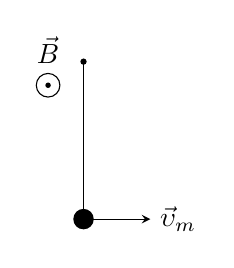
\begin{tikzpicture}[>=stealth]

\draw (0,2)--(0,0);\fill (0,2) circle(.04) (0,0) circle(.13);
\draw (-.45,1.7) circle(.15) node[above=.15cm]{$\vec B$};\fill (-.45,1.7) circle(.035);
\draw[->] (0,0)--(.85,0) node[right]{$\vec\upsilon_m$};
\end{tikzpicture}\end{center}
В однородном магнитном поле вращается по окружности в вертикальной плоскости положительно заряженный шарик массой m и зарядом q. Длина нити равна l. Минимальная скорость шарика в нижней точке, при которой шарик сможет совершить полный оборот, равна \ensuremath{\upsilon}. Найдите индукцию магнитного поля B.
}{
\smallskip\noindent\textbf{Решение}\par
\begin{center}\begin{tikzpicture}[>=stealth]

\draw (0,0) circle(1.4) (0,-1.4)--(0,1.4);\fill (0,-1.4) circle(.07) (0,0) circle(.05) (0,1.4) circle(.07);
\draw[->] (0,1.4)--(0,2.25) node[right]{$\vec F_{\!\text{л}}$};\draw[->] (0,1.4)--(0,.82) node[right]{$m\vec g$};
\draw[->] (0,.67)--(0,.29) node[right]{$\vec a$};\draw[->] (0,1.4)--(-.85,1.4) node[left]{$\vec\upsilon_2$};
\draw[->] (0,-1.4)--(.85,-1.4) node[right]{$\vec\upsilon_1$};\fill (-1.85,1.4) circle(.04) node[right]{$\vec B$};
\end{tikzpicture}\end{center}
При движении положительно заряженного тела магнитное поле действует на него с силой Лоренца, равной $F_{\,\text{л}}=Bq v \sin \alpha ,$ где $\sin \alpha =1,$ направление которой определяется правилом левой руки.
Рассмотрим движение заряженного шарика в магнитном и гравитационном поле. За нулевой уровень высоты примем нижнюю точку расположения шарика. В нижней точке он обладает кинетической энергией $E_{\,\text{к}1}= \frac{m v _1 ^2}{2} ,$  в верхней  — кинетической $E_{\,\text{к}2}= \frac{m v _2 ^2}{2}$ и потенциальной $E_{\,\text{п}2}=mgh=2mgl,$ где $v _2$ — скорость шарика в верхней точке. 
Так как сила Лоренца перпендикулярна вектору скорости, то работу не совершает. Тогда применим закон сохранения энергии:

\[\frac{m v _1 ^2}{2} = \frac{m v _2 ^2}{2} + 2mgl. ( 1 )\]

Так как шарику придали минимальную скорость, чтобы он совершил оборот в вертикальной плоскости, то в верхней точке сила натяжения нити равна $0$. На шарик в верхней точке действуют сила тяжести, сила Лоренца, направленная вверх. Под действием этих сил шарик имеет в верхней точке центростремительное ускорение $a= \frac{v _2 ^2}{R} = \frac{v _2 ^2}{l} .$
По второму закону Ньютона $m \vec{g} + \vec F_{\,\text{л}}=m \vec{a}.$ В проекции на вертикальную ось, направленную вниз получаем:

$mg - F_{\,\text{л}}=ma$
$Bq v _2=mg - \frac{m v _2 ^2}{l} . ( 2 )$

Объединяя формулы ($1$) и ($2$), находим индукцию магнитного поля:

\[B= \frac{m ( 5gl - v _1 ^2 )}{ql \sqrt{v _1 ^2 - 4gl}} .\]

Ответ: $B= \frac{m ( 5gl - v _1 ^2 )}{ql \sqrt{v _1 ^2 - 4gl}}$
}

% Source 35160: https://phys-ege.sdamgia.ru/problem?id=35160
\BankTask{35160}{
Шар массой $1\,\text{кг}$, подвешенный на нити длиной $90\,\text{см}$, отводят от положения равновесия на угол $60$° и отпускают. В момент прохождения шаром положения равновесия в него попадает пуля массой $10\,\text{г}$, летящая навстречу шару. Она пробивает его и продолжает двигаться горизонтально. Определите модуль изменения импульса пули в результате попадания в шар, если он, продолжая движение в прежнем направлении, отклоняется на угол $39$°. (Массу шара считать неизменной, диаметр шара  — пренебрежимо малым по сравнению с длиной нити, $\cos 39 ^\circ = \frac{7}{9} .$) Какие законы Вы используете для решения задачи? Обоснуйте их применение.
}{
\smallskip\noindent\textbf{Решение}\par
Обоснование
$1$.  Введем инерциальную систему отсчета (ИСО), связанную с Землей.
$2$.  Тела движутся поступательно, размеры шарика малы по сравнению с размером нити, поэтому шарик и пулю можно описывать моделью материальной точки.
$3$.  Будем считать время взаимодействия пули и шарика малым, чтобы нить за время соударения не успела заметно отклониться. Тогда все силы в момент соударения направлены вертикально. Следовательно, в ИСО при попадании пули в шарик сохраняется горизонтальная составляющая импульса системы «шарик + пуля».
$4$.  После попадания пули в шарик при движении тел по вертикальной окружности механическая энергия равна сумме кинетической и потенциальной энергий тел $E=E_{\,\text{п}} + E_{\,\text{к}}.$ Изменение механической энергии тел в ИСО равно работе всех непотенциальных сил, приложенных к телу. Работа непотенциальной силы натяжения нити равна нулю, так как сила натяжения направлена перпендикулярно скорости в любой точке траектории.
$5$.  За нулевой уровень потенциальной энергии примем уровень положения равновесия шарика.

Перейдем к решению.
Потенциальная энергия равна $E_{\,\text{п}}=Mgh=Mgl ( 1 - \cos \alpha ) .$
Кинетическая энергия шарика в нижней точке $E_{\,\text{к}}= \frac{M v _0 ^2}{2} .$
По закону сохранения энергии:

\[Mgl ( 1 - \cos \alpha ) = \frac{M v _0 ^2}{2} .\]

Тогда скорость шарика в нижней точке равна:

\[v _0= \sqrt{2gl ( 1 - \cos \alpha )} .\]

Запишем законы сохранения импульса в момент удара и закон сохранения энергии после удара и до подъема шарика на максимальную высоту:

\[\begin{cases}Mv_0-mv_1=Mu-mv_2,\\ \dfrac{Mu^2}{2}=Mgl(1-\cos\beta).\end{cases}\]

Находим скорость шарика сразу после удара:

\[u= \sqrt{2gl ( 1 - \cos \beta )} .\]

Тогда изменение скорости пули равно:

$|\Delta v | = v _1 - v _2= \frac{M \sqrt{2gl}}{m} ( \sqrt{1 - \cos \alpha} - \sqrt{1 - \cos \beta} ) ;$
$|\Delta v|=\frac{1\cdot\sqrt{2\cdot10\cdot0{,}9}}{0{,}01}\left(\sqrt{1-0{,}5}-\sqrt{1-\frac79}\right)=100\,\text{м/с}.$

Модуль изменения импульса пули равен:

\[|\Delta p|=m|\Delta v |=0{,}01 \cdot 100=1 \,\text{кг} \cdot \,\text{м/с} .\]

Ответ: $1 \,\text{кг} \cdot \,\text{м/с} .$
}

% Source 25758: https://phys-ege.sdamgia.ru/problem?id=25758
\BankTask{25758}{
Небольшая шайба после удара скользит вверх по наклонной плоскости из точки А (см. рис.).
\begin{center}\begin{tikzpicture}[task graph,>=stealth]\draw (0,0)--(5.8,0);\draw (0,0)--(4.5,1.38) arc (107:0:1.04);\draw (1,0) arc (0:17:1) node[midway,right]{\(\alpha\)};\begin{scope}[rotate=17]\draw[fill=gray!15] (0,0) rectangle(.85,.45);\draw[->](.85,.23)--(2,.23)node[above left]{\(\vec v_0\)};\end{scope}\node[below]at(0,0){\(A\)};\node[above]at(4.5,1.38){\(B\)};\draw[->](4.8,.39)--(5.55,1.12)node[midway,below right]{\(R\)};\end{tikzpicture}\end{center}
В точке В наклонная плоскость без излома переходит в наружную поверхность горизонтальной трубы радиусом R. Если в точке А скорость шайбы превосходит $v _0=4\,\text{м/с},$ то в точке В шайба отрывается от опоры. Длина наклонной плоскости $AB=L=1\,\text{м},$ угол $\alpha = 30 ^\circ.$ Коэффициент трения между наклонной плоскостью и шайбой $\mu =0{,}2.$ Найдите внешний радиус трубы R.
Какие законы Вы использовали для описания движения тела? Обоснуйте их применимость к данному случаю.
}{
\smallskip\noindent\textbf{Решение}\par
Обоснование 
$1$.  Рассмотрим задачу в системе отсчета, связанной с Землей. Будем считать эту систему отсчета инерциальной (ИСО). 
$2$.  Шайбу описываем моделью материальной точки, так как его размерами в данных условиях можно пренебречь.
$3$.  Поступательное движение шайбы происходит по шероховатой поверхности, поэтому на нее действует сила трения скольжения, равная $F_{\,\text{тр}}=\mu N.$
$4$.   На тело действуют потенциальная сила тяжести, сила реакции опоры и непотенциальная сила трения. Поскольку шайба описывается моделью материальной точки, то при движении тела по наклонной плоскости в ИСО работа силы трения равна изменению механической энергии.
$5$.  Для материальной точки условие отрыва шайбы от поверхности формулируется на основе второго закона Ньютона. В момент отрыва обращается в ноль сила реакции опоры. 
$6$.  В точке отрыва на тело действует только сила тяжести, которая является причиной ускорения свободного падения, направленного вертикально вниз и равная $10\,\text{м/с}^{2}$. Это же ускорение является центростремительным. Для модели материальной точки в ИСО применимы законы движения по окружности.

Перейдем к решению. 
По закону сохранения энергии в незамкнутой системе:

\[A_{\,\text{тр}}= E_{\,\text{пол}2} - E_{\,\text{пол}1},\]

где полная энергия в первом состоянии $E_{\,\text{пол}1}=E_{\,\text{к}1}= \frac{m v _0 ^2}{2} ,$ полная энергия во втором состоянии $E_{\,\text{пол}2}=E_{\,\text{к}2} + E_{\,\text{п}2}= \frac{m v _{\,\text{в}} ^2}{2} + mgh,$ причем высота подъема тела $h=L \sin \alpha .$ Работа силы трения $A_{\,\text{тр}}= - F_{\,\text{тр}}L,$ при этом сила трения скольжения $F_{\,\text{тр}}=\mu N.$ Из проекции на ось Oy $N=mg \cos \alpha .$
Объединяя формулы, получаем:

$\frac{m v _0 ^2}{2} =\mu mgL \cos \alpha + \frac{m v _B ^2}{2} + mgL \sin \alpha .$ ($1$)

В точке В условием отрыва будет равенство центростремительного ускорения $a= \frac{v _{\,\text{в}} ^2}{R}$ величине нормальной составляющей ускорения свободного падения:

$\frac{v _B ^2}{R} =g \cos \alpha ,$  откуда $v _B ^2 =Rg \cos \alpha .$($2$)

Из ($1$) и ($2$) находим внешний радиус трубы R:

\[R= \frac{v _0 ^2}{g \cos \alpha} - 2L ( \mu + \tan \alpha ) = \frac{16}{10 \cdot \cos 30 ^\circ} - 2 \cdot 1 \cdot ( 0{,}2 + \tan 30 ^\circ ) \approx 0{,}3\,\text{м}.\]

Ответ: R  =  $0{,}3\,\text{м}$.
}

% Source 29761: https://phys-ege.sdamgia.ru/problem?id=29761
\BankTask{29761}{
На горизонтальной поверхности неподвижно закреплена абсолютно гладкая полусфера радиусом $R=2{,}5$ м. С ее верхней точки из состояния покоя соскальзывает маленькое тело. В некоторой точке тело отрывается от сферы и летит свободно. Найдите скорость тела в момент отрыва от сферы. Сопротивлением воздуха пренебречь. Обоснуйте применимость используемых законов к решению задачи.
}{
\smallskip\noindent\textbf{Решение}\par
Обоснование
Систему отсчета, связанную с Землей, будем считать инерциальной. Поскольку размеры тела, соскальзывающего с полусферы, малы, то его можно считать материальной точкой. При движении тела от вершины полусферы выполняется закон сохранения механической энергии, так как полусфера гладкая, и работа силы реакции опоры равна нулю (эта сила перпендикулярна скорости тела). В момент отрыва обращается в ноль сила реакции опоры $\vec N .$ Второй закон Ньютона выполняется в ИСО для модели материальной точки.

Перейдем к решению.
$1$.  Рассмотрим два состояния системы  — в верхней точке полусферы и в точке отрыва от поверхности. В верхней точке шарик обладает потенциальной энергией $E_{p1}=m g h_1,$ причем $h_1=R.$ В точке отрыва от поверхности шарик обладает кинетической энергией $E_{k2}= \frac{m v ^2}{2}$ и потенциальной энергией $E_{p2}=m g h.$ Шарик при движении не вращается вследствие отсутствия силы трения, поэтому кинетической энергией вращения можно пренебречь.
По закону сохранения энергии:

\[m g R= \frac{m v ^2}{2} + m g h.\]

$2$.  Шарик отрывается от поверхности полусферы в том случае, когда сила реакции опоры становится равной нулю. На шарик действует сила тяжести, при движении по окружности ускорение направлено к центру окружности. Тогда по второму закону Ньютона в проекции на ось, совпадающую с вектором ускорения, получаем: $m a=m g \cos \alpha .$ Из рисунка видно, что $\cos \alpha = \frac{h}{R} .$ \begin{center}\begin{tikzpicture}[task graph,>=stealth]\draw(-2.04,0)--(3.08,0);\draw(1.6,0)arc(0:180:1.6);\draw(0,0)--(0,1.6)node[midway,left]{\(R\)};\filldraw[fill=gray!15](0,1.68)circle(.09) (1.13,1.13)circle(.09);\draw[dashed](0,0)--(1.13,1.13);\draw(1.13,1.13)--(3.08,1.13);\draw[<->](2.82,0)--(2.82,1.13)node[midway,right]{\(h\)};\draw(1.13,.8)arc(270:225:.33)node[midway,below left]{\(\alpha\)};\draw[->] (1.13,1.13)--(.49,.49) node[left]{\(\vec a\)};\draw[->] (1.13,1.13)--(1.13,-.55) node[right]{\(m\vec g\)};\end{tikzpicture}\end{center}
$3$.  При движении по окружности центростремительное ускорение равно $a= \frac{v ^2}{R} .$ 
$4$.  Объединяя формулы и решая совместно уравнения, выражаем скорость шарика в момент отрыва:

\[v = \sqrt{\frac{2 g R}{3}} = \sqrt{\frac{2 \cdot 10 \cdot 2{,}5}{3}} \approx 4{,}1 \,\text{м/с}.\]

Ответ: $4{,}1\,\text{м/с}$.
}

\end{document}
